\section{Characteristics}
\label{sec:characteristics}

% Characteristics are used to describe the position of a fact along a dimension.
% Some of them rely on report elements for description, while others introduce new concepts. 
% All characteristics share a common interface \texttt{ICharacteristic}.
% Each characteristic acts as a aspect-value pair, 
% where the aspect characterizes the dimension's axis and the value details the position of the fact along the axis.
% The interplay between aspect and characteristics classes is illustrated in figure \ref{fig:characteristics}.
Characteristics serve to pinpoint a fact's location within a dimension. 
They utilize report elements for their descriptions or introduce novel, separate characteristics.
All characteristics are unified under the \texttt{ICharacteristic} interface. 
Every characteristic functions as an aspect-value duo, 
with the aspect defining the dimension's axis and the value specifying the fact's location on that axis. 
The dynamic between aspects and characteristics is depicted in figure \ref{fig:characteristics}.

\begin{figure}[H]
    \centering
    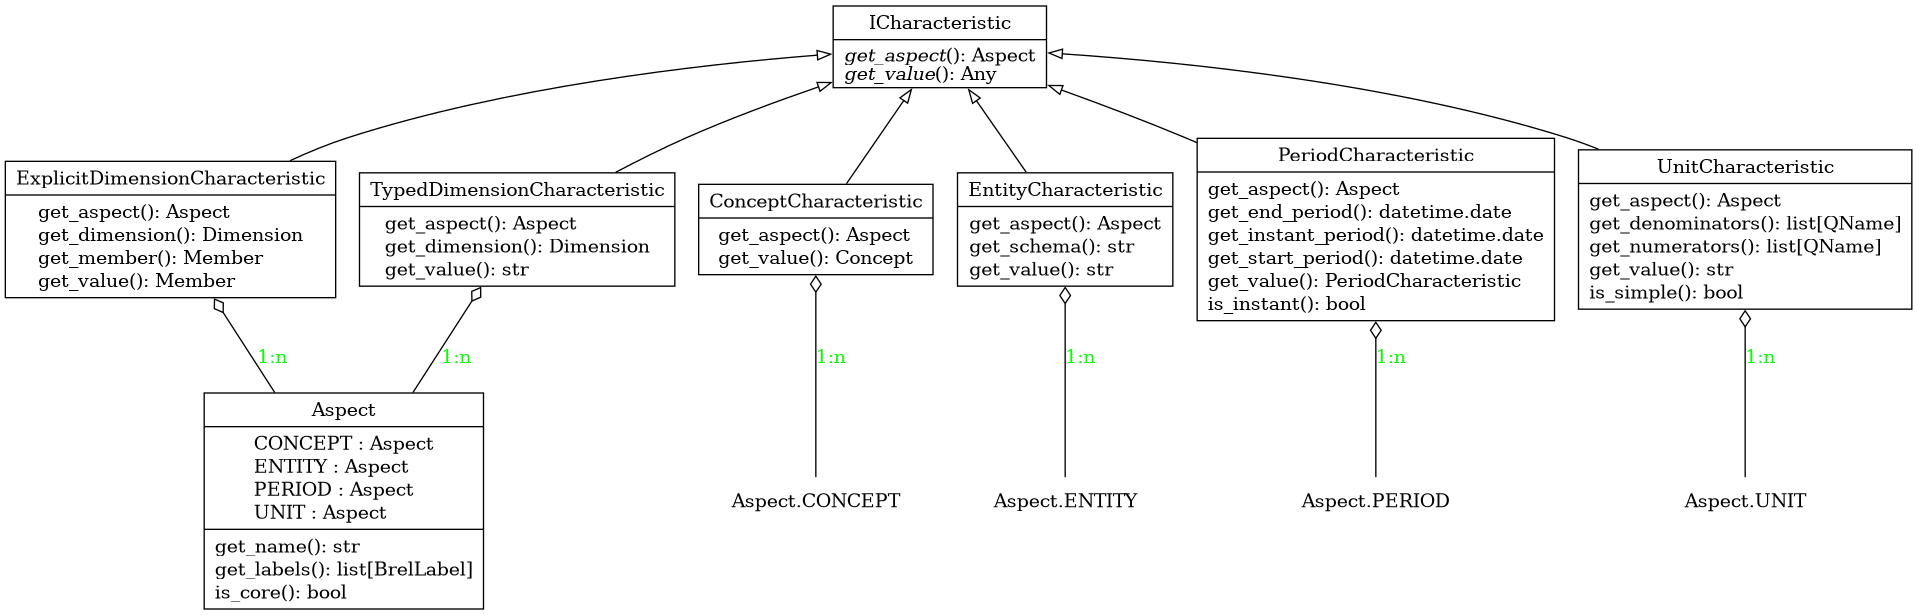
\includegraphics[width=\textwidth]{images/brel_characteristics_classes.png}
    \caption{The interplay between aspects and characteristics}
    \label{fig:characteristics}
\end{figure}

% The \texttt{ICharacteristic} interface is integral to the Brel API, which is why it is described first.
% Next up is the Aspect class, followed by the different types of characteristics.

\subsection{ICharacteristic}

% As I have pointed out in the previous section, characteristics are used to describe the position of a fact along a dimension using an aspect-value pair.
% An aspect is a description of the dimension's axis, while the value details the position of the fact along the axis.
As mentioned earlier, characteristics describe a fact's dimensional location through an aspect-value combination.
Here, the aspect describes the dimension's axis, and the value conveys the fact's precise location on the axis.

% The \texttt{ICharacteristic} interface follows this definition directly by providing the methods \texttt{get\_aspect} and \texttt{get\_value}.
Directly aligning with this concept, 
the \texttt{ICharacteristic} interface offers the methods \texttt{get\_aspect} and \texttt{get\_value}.

\subsection{Aspect}

% Aspects are used to describe the axis of a dimension.
% Each instance of the \texttt{Aspect} class represents a single aspect.
% The core aspects - Concept, Entity, Period and Unit - are all instances of the \texttt{Aspect} class.
% In addition, the core aspects are statically available as public constants of the \texttt{Aspect} class.
% The fields in question are \texttt{Aspect.CONCEPT}, \texttt{Aspect.ENTITY}, \texttt{Aspect.PERIOD} and \texttt{Aspect.UNIT}.

% The \texttt{Aspect} class provides a method for getting the name of the aspect, called \texttt{get\_name}.
% The name of an aspect is a string instead of the QName class.
% The main reason for this is that the core aspects are available globally without the use of namespaces.
% Most facts exclusively use the core aspects.
% So the namespaces of QNames would only add unnecessary clutter.
% The only exception to this rule are dimensions, where the name of the dimension is a QName.
% Still, QNames can just be emulated by using strings using their expanded name format.

Aspects define the axes of dimensions.
Each \texttt{Aspect} class instance corresponds to a unique aspect.
The primary aspects - Concept, Entity, Period, and Unit - are represented as instances of the \texttt{Aspect} class.
Moreover, these core aspects are accessible as public constants within the \texttt{Aspect} class,
specifically through the fields \texttt{Aspect.CONCEPT}, \texttt{Aspect.ENTITY}, \texttt{Aspect.PERIOD}, and \texttt{Aspect.UNIT}.

The \texttt{Aspect} class includes a method named \texttt{get\_name} for retrieving an aspect's name,
% which returns a string representation rather than using the QName class.
which returns a string.
% This approach is adopted because the core aspects are globally recognized without necessitating namespaces,
% simplifying the representation as most facts primarily involve these core aspects.
% Incorporating namespaces via QNames would only complicate matters unnecessarily.
% Dimensions represent the sole exception to this guideline, utilizing QNames for dimension names.
% Nevertheless, QNames are effectively simulated through strings in their expanded name format for consistency and simplicity.
% \footnote{The expended name format of a QName is \texttt{namespace\_prefix:local\_name}.\cite{w3_expanded_names}}
% \cite{w3_qnames}

% Similar to the \texttt{IReportElement} interface, the \texttt{Aspect} class also provides a method for getting the label of the aspect.
% The \texttt{get\_labels} method returns a list of labels, since an aspect can have multiple labels.

% Finally, the \texttt{is\_core} method returns whether the aspect is a core aspect or not.
Just like the \texttt{IReportElement} interface, the \texttt{Aspect} class incorporates a method to obtain the label of the aspect.
The method \texttt{get\_labels} produces a collection of labels because an aspect might possess several labels.

Moreover, the \texttt{is\_core} function determines if an aspect belongs to the category of core aspects.

% \subsection{Concept Characteristic}

% The \texttt{ConceptCharacteristic} indicates which concept a fact uses.
% From the perspective of hypercubes, the \texttt{Aspect.CONCEPT} aspect is a dimension of concepts 
% and the actual \texttt{Concept} report element is a point along that dimension.
% The dimension characteristic is the only characteristic that every context has to have.

% The \texttt{ConceptCharacteristic} implements \texttt{ICharacteristic} as one would expect.
% \texttt{get\_aspect} returns \texttt{Aspect.CONCEPT} and \texttt{get\_value} returns the concept that the characteristic describes.
\subsection{Concept Characteristic}

The \texttt{ConceptCharacteristic} specifies the concept employed by a fact.
In the context of hypercubes, \texttt{Aspect.CONCEPT} serves as a dimension encompassing various concepts,
while the specific \texttt{Concept} report element represents a point within this dimension.
It is essential for every context to include this dimension characteristic.

As expected, the \texttt{ConceptCharacteristic} adheres to the \texttt{ICharacteristic} interface.
\texttt{get\_aspect} yields \texttt{Aspect.CONCEPT}, and \texttt{get\_value} returns the \texttt{Concept} instance.

% \subsection{Entity Characteristic}

% The \texttt{EntityCharacteristic} dictates which entity a fact belongs to.
% From the perspective of hypercubes, the \texttt{Aspect.ENTITY} aspect is a dimension of entities
% An entity is a legal entity, such as a company and
% can be identified by a tag and a scheme\footnote{Schemes tend to be URLs.} that acts as the namespace of the tag.
% Both of these values are combined into a single string using the notation \texttt{\{scheme\}tag}.\footnote{The notation is similar to the Clark notation for QNames.\cite{w3_qnames}}

% The \texttt{EntityCharacteristic} implements the \texttt{ICharacteristic} interface,
% where \texttt{get\_aspect} returns \texttt{Aspect.ENTITY} and \texttt{get\_value} gives the string representation of the entity as described above.
\subsection{Entity Characteristic}

The \texttt{EntityCharacteristic} identifies the entity associated with a fact.
% Within hypercube structures, the \texttt{Aspect.ENTITY} aspect categorizes dimensions of entities,
An entity, such as a corporation, is distinguished by a tag and a scheme\footnote{Schemes are typically URLs.} serving as the tag's namespace.
These identifiers are merged into a singular string format \texttt{\{scheme\}tag},
\footnote{This format mirrors the Clark notation used for QNames.\cite{w3_qnames}}

Implementing the \texttt{ICharacteristic} framework,
\texttt{get\_aspect} returns \texttt{Aspect.ENTITY} and \texttt{get\_value} provides the entity's string representation as previously mentioned.

\subsection{Period Characteristic}

The \texttt{PeriodCharacteristic} specifies the time frame of a fact.
Periods can be either instant or duration, which can be checked using the \texttt{is\_instant} method.

The methods \texttt{get\_start\_date} and \texttt{get\_end\_date} return the start and end date of a duration period respectively.
% If the period is instant, the methods raise an exception, since instant periods do not have a start or end date.
Should the period be an instant, these methods will trigger an exception, highlighting that instant periods lack defined start or end points.
Conversely, the method \texttt{get\_instant} returns the instant of the period.
If the period is duration, the method raises an exception, since duration periods do not have an instant.
% All three methods return a date of type \texttt{datetime.date}, which is a standard Python class for representing dates.
% Again, period characteristics implement the \texttt{ICharacteristic} interface.
% \texttt{get\_aspect} returns \texttt{Aspect.PERIOD} and \texttt{get\_value} returns the period characteristic itself.
% The reason why \texttt{get\_value} returns itself is that there is no basic type for representing XBRL periods in python.
% The python \texttt{datetime} module, which is the de-facto standard for representing dates in python, 
% does not provide a class for representing both instant and duration periods in a single class. 
Each of the three methods yields a date of the type \texttt{datetime.date}, which is a conventional Python class used for date representation.

Additionally, period characteristics conform to the \texttt{ICharacteristic} interface. 
\texttt{get\_aspect} emits \texttt{Aspect.PERIOD} and \texttt{get\_value} returns the period characteristic itself. 
The justification for \texttt{get\_value} delivering the characteristic itself stems from the lack of a primitive type in Python to represent XBRL periods. 
The Python \texttt{datetime} module, regarded as the standard for date depiction in Python, 
does not offer a class that represents both instant and duration periods together.

\subsection{Unit Characteristic}

% The \texttt{UnitCharacteristic} describes the unit of a fact.
% Like all other characteristics before it, the \texttt{UnitCharacteristic} represents a point along the unit dimension 
% and it implements the \texttt{ICharacteristic} interface.
% From a semantic point of view, the unit characteristic also defines the type of the fact's value.
% A fact with a unit of \texttt{USD} has a value of type \texttt{decimal} and a fact with a unit of \texttt{date} has a value representing a date.

% Units come in one of two forms - simple and complex.
% Simple units are atomic units, such as \texttt{USD} or \texttt{shares}.
% Complex units are composed of multiple simple units, such as \texttt{USD per share}.
% All complex units are formed by dividing one or more simple units by zero or more simple units.
The \texttt{UnitCharacteristic} specifies the unit of a fact and adheres to the \texttt{ICharacteristic} interface.
Semantically, the unit characteristic further determines the fact's value type.
A fact assigned with a \texttt{USD} unit is of the \texttt{decimal} type, whereas a fact with a \texttt{date} unit signifies a date value.

Units are categorized into two types: simple and complex.
Simple units are indivisible, exemplified by \texttt{USD} or \texttt{shares}.
Complex units consist of multiple simple units combined, such as \texttt{USD per share}.
Each complex unit is constructed by dividing one or more simple units by another set of simple units.

\begin{figure}[H]
    \centering
    \caption{Schematic of composition of complex units}
    $$\frac{num\_unit_1 \cdot num\_unit_2 \cdot ...}{1 \cdot denom\_unit_1 \cdot denom\_unit_2 \cdot ...}$$
    \label{fig:complex_unit}
\end{figure}

% Brel represents the complex unit in figure \ref{fig:complex_unit} using two lists of simple units.
% The method \texttt{get\_numerators} returns the list of simple units in the numerator, \texttt{get\_denominators} returns the denominators.\footnote{The returned list of denominators does not contain the implicit denominator of 1.}
Brel depicts the complex unit in figure \ref{fig:complex_unit} through a pair of lists containing simple units.
The function \texttt{get\_numerators} delivers the numerator's list of simple units, while \texttt{get\_denominators} yields the list of denominators
\footnote{The list of denominators provided excludes the implicit denominator of 1.}.

Similar to the \texttt{PeriodCharacteristic}, the method \texttt{get\_value} of the \texttt{UnitCharacteristic} returns the characteristic itself.

% Similar to the \texttt{PeriodCharacteristic}, the \texttt{UnitCharacteristic} does not have a basic type for representing XBRL units.
% Instead, it returns itself when \texttt{get\_value} is called.
% The method \texttt{get\_aspect} returns \texttt{Aspect.UNIT} as expected.
% TODO: Make unit characteristic get_value return itself in code base

\subsection{Dimension Characteristics}

% There are two categories of dimension characteristics in XBRL - typed and explicit.
XBRL differentiates between two types of dimension characteristics: typed and explicit.
The two types are represented by the \texttt{TypedDimensionCharacteristic} and \texttt{ExplicitDimensionCharacteristic} classes respectively.
% Typed dimension characteristics are used to describe a custom axis, along which a fact is positioned.
% The kind of values along this custom axis are of a specific type.
Like every other characteristic, both implement the \texttt{ICharacteristic} interface.

% As we have seen in section \ref{sec:api_report_elements}, custom dimensions are represented as a \texttt{Dimension} report element in Brel.
As discussed in section \ref{sec:api_report_elements}, Brel models custom dimensions as \texttt{Dimension} report elements.
Accordingly, the aspect of a dimension characteristic should represent a \texttt{Dimension} report element.
% Luckily, \texttt{Dimension} objects are essentially just a name, which is represented by a QName.
Therefore, the \texttt{get\_aspect} method of both classes returns the QName of the \texttt{Dimension} instance as a string.

% The characteristic also provides direct access to the \texttt{Dimension} object itself via the \texttt{get\_dimension} method.
% Think of \texttt{get\_dimension} as a more complete version of \texttt{get\_aspect}.
Dimension characteristics facilitate direct access to the \texttt{Dimension} object itself through the \texttt{get\_dimension} method.
% View \texttt{get\_dimension} as an elaborated form of \texttt{get\_aspect}.

As the name suggests, the value of a typed dimension characteristic pertains to a specific type.
The \texttt{get\_value} method should reflect this accordingly.
It should return the value in a type that encompasses all possible values of the dimension.
The most general type of any value in XBRL is a string.

The actual type of the value is determined by the \texttt{get\_type} method of the \texttt{Dimension} element.
\footnote{The \texttt{Dimension} object returned by \texttt{get\_dimension} is guaranteed to be a typed dimension with \texttt{is\_explicit} returning \texttt{False}.}
% Naturally, Brel provides helper methods for converting the value into the type that most appropriately represents the value.
% These helper methods are not part of the minimal API described in this chapter, but they are part of the full API.
Brel includes auxiliary methods designed to convert the value into the format that best reflects its intended representation.
While these helper methods are not included within the minimal API outlined in this chapter, they are part to the comprehensive API.

Explicit dimensions are the second category of custom characteristic.
They are extremely similar to typed dimensions, but they do not have a type.
Instead of a type, they have a set of possible values.

The \texttt{ExplicitDimensionCharacteristic} class is almost identical to the \texttt{TypedDimensionCharacteristic} class.
The main difference between the two is that \texttt{get\_value} returns a \texttt{Member} object instead of a string.

